\begin{solution}{normal}
If the water was displaced a small distance $s$ from equilibrium (distance $|AB|$), the surface tension forces would have to cancel out by the principal of virtual work.
\begin{center}
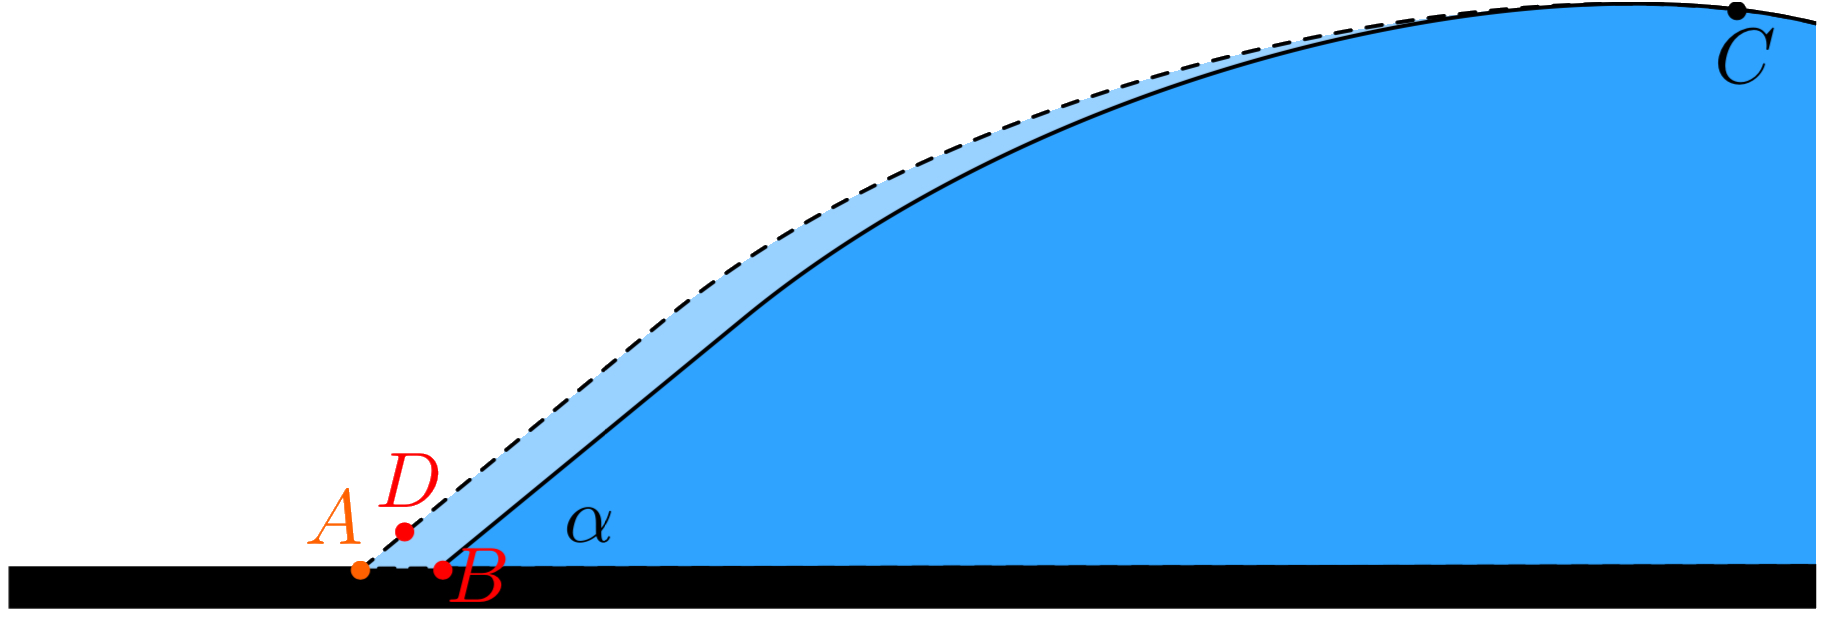
\includegraphics[width=15cm]{pool.png}
\end{center}
This means that 
\[\sigma s + \sigma s' = 0\]
where $s'$ is the distance the water has expanded (distance $|AD|$) after moving away a distance $s$ from equilibrium. We express the total energy as 
\[E = \sigma S + \sigma' S + mg\frac{h}{2}\]
where $S$ is the surface area, $m$ is the mass of the puddle, and $h = V/S$ is the thickness of the puddle. We then substitute these relations to get 
\[E = \sigma S(1 - \cos\theta) + \frac{\rho g V^2}{2S}.\]
Minimizing this function for $E$ gives us 
\[\frac{dE}{dS} = \sigma (1 -\cos\theta) - \frac{\rho gV^2}{2S^2} = 0\implies S = \sqrt{\frac{\rho gV^2}{2\sigma (1 - \cos\theta)}}.\]
Note that $h = V/S$, therefore, 
\[h = \frac{V}{S} = \boxed{\sqrt{\frac{2\sigma}{\rho g} (1 -\cos\theta)}}.\]
\tcbline 
\textbf{Solution 2.} We consider equilibrium of the surface defined by the two endpoints $\text{B}$ and $\text{C}$ in the figure of the solution before. There will be two surface tension forces directed at both endpoints of magnitude $\sigma x$ where $x$ is the total length of the surface. Taking forces into horizontal equilibrium gives us 
\[\sigma x (1 - \cos\alpha) = \int P x \cdot ds\sin\alpha = \int Pxdy\]
where $P$ is the external pressure.  Taking this result into account tells us that 
\begin{align*}
\sigma x (1-\cos\alpha) &= \int_{0}^{h} \rho gy xdy\\
\sigma (1-\cos\alpha) &= \frac{1}{2}\rho gy^2\implies y = \boxed{\sqrt{\frac{2\sigma}{\rho g} (1 -\cos\alpha)}}
\end{align*}
\blfootnote{It is believed that the symbolic answer to this problem is incorrect as the same answer derived here is given in \hyperlink{https://en.m.wikipedia.org/wiki/Surface_tension#Puddles_on_a_surface}{Wikipedia}}
\end{solution}